%%%%%%%%%%%%%%%%%%%%%%%%%%%%%%%%%%%%

\section{1.3. Coleta dos dados}

%%%%%%%%%%%%%%%%%%%%%%%%%%%%%%%%%%%%

\subsection{Populações e amostras}

%%%%%%%%%%%%%%%%%%%%%%%%%%%%%%%%%%%%

\begin{frame}
\frametitle{Populações e amostras}


\begin{center}
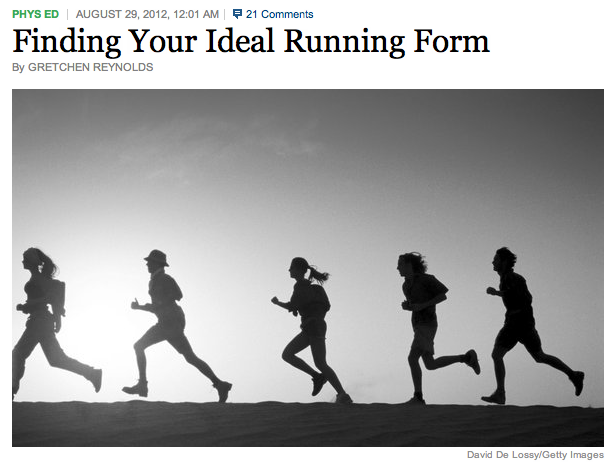
\includegraphics[width=0.5\textwidth]{1-3_data_collection_principles/figures/running.png}
\end{center}
\vspace{-0.5cm}
{\tiny \webURL{http://well.blogs.nytimes.com/2012/08/29/finding-your-ideal-running-form}}

\vspace{1cm}
\small{\textit{Tradução: Encontre sua corrida ideal.}}

\end{frame}
%%%%%%%%%%%%%%%%%%%%%%%%%%%%%%%%%%%%

\begin{frame}
\frametitle{Populações e amostras}
{
\justifying
\hl{Questão de pesquisa:} As pessoas podem se tornar corredores melhores e mais eficientes sozinhos, simplesmente correndo? \\
}
\vspace{0.5cm}
{
\justifying
\pause 
\justifying
\hl{População de interesse:} \soln{\pause Todas as pessoas.}
}
\pause 
\justifying
$\:$ \\
\vspace{0.5cm}
\justifying
\hl{Amostra:} Grupo de mulheres adultas que se juntaram recentemente a um grupo de corrida.\\
\vspace{0.5cm}
\pause
\justifying
\hl{População para a qual os resultados podem ser generalizados:} \soln{\pause Mulheres adultas, se os dados forem amostrados aleatoriamente.}

\end{frame}

%%%%%%%%%%%%%%%%%%%%%%%%%%%%%%%%%%%%

\subsection{Evidência anedótica}

%%%%%%%%%%%%%%%%%%%%%%%%%%%%%%%%%%%%

\begin{frame}
\frametitle{Evidência anedótica e pesquisa precoce sobre tabagismo}

\begin{itemize}
\justifying
\item A pesquisa antifumo começou nas décadas de 1930 e 1940, quando o consumo de cigarros se tornou cada vez mais popular. Enquanto alguns fumantes pareciam ser sensíveis à fumaça do cigarro, outros não eram afetados.
\vspace{0.5cm}
\justifying
\item A pesquisa anti-tabagismo foi confrontada com uma resistência baseada em \hl{evidências anedóticas} como "Meu tio fuma três maços por dia e está em perfeita saúde", evidência baseada em um tamanho de amostra limitado que pode não ser representativo da população.

\end{itemize}
\end{frame}

%%%%%%%%%%%%%%%%%%%%%%%%%%%%%%%%%%%%
\begin{frame}
\frametitle{Evidência anedótica e pesquisa precoce sobre tabagismo (cont.)}

\begin{itemize}
\justifying
\item Concluiu-se que "fumar é um comportamento humano complexo, por sua natureza difícil de estudar, confundido pela variabilidade humana".
\vspace{0.5cm}
\justifying
\item Com o tempo, os pesquisadores puderam examinar amostras maiores de casos (fumantes), e as tendências mostrando que fumar tem impactos negativos na saúde se tornaram muito mais claras.

\end{itemize}

\ct{Brandt, \textit{O século do cigarro} (2009), Livro Básico.}

\end{frame}

%%%%%%%%%%%%%%%%%%%%%%%%%%%%%%%%%%%%

\subsection{Amostragem de uma população}

\begin{frame}
\frametitle{Censo}

\begin{itemize}

\item Não seria melhor "amostrar" toda a população?

\begin{itemize}
\item Isso é chamado de \hl{censo}.
\end{itemize}

\pause

\item Há problemas em realizar um censo:

\begin{itemize}
\justifying
\item Pode ser difícil concluir um censo: sempre parece haver pessoas difíceis de localizar ou difíceis de avaliar. \textit{E essas pessoas difíceis de encontrar podem ter certas características que as distinguem do resto da população.}

\justifying
\item Populações raramente ficam paradas. Mesmo se você pudesse fazer um censo, a população muda constantemente, então nunca é possível obter uma medida perfeita.
\justifying
\item Fazer um censo pode ser mais complexo que a amostragem.
\end{itemize}

\end{itemize}

\end{frame}

%%%%%%%%%%%%%%%%%%%%%%%%%%%%%%%%%%%%%

\begin{frame}
\frametitle{Censo (cont.)}
\vfill

\begin{center}
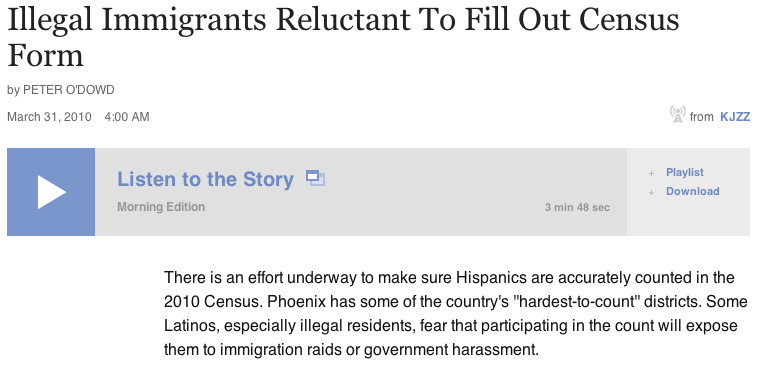
\includegraphics[width=0.50\textwidth]{1-3_data_collection_principles/figures/census_illegal_immig.png}
\end{center}

\ct{\webURL{http://www.npr.org/templates/story/story.php?storyId=125380052}}\\


\justifying
\small{
\hl{Tradução título:} Imigrantes ilegais relutam em preencher o formulário de recenseamento.\\
\justifying
\hl{Tradução texto:} Há uma pesquisa que busca  garantir que os hispânicos sejam contados com precisão no censo de 2010. Phoenix tem alguns dos distritos mais difíceis de serem pesquisados. Alguns latinos, especialmente moradores ilegais, temem que a participação na contagem os exponha a incursões na imigração ou a assédio do governo.}
\end{frame}

%%%%%%%%%%%%%%%%%%%%%%%%%%%%%%%%%%%%%

\begin{frame}
\frametitle{Análise exploratória e inferência}

\begin{itemize}

\item A amostragem é natural.

\pause

\justifying
\item Pense em provar algo que você está cozinhando - você prova (examina) uma pequena parte do que está cozinhando para ter uma ideia do prato como um todo.

\pause

\justifying
\item Quando você provar uma colherada de sopa e decidir que nesta colherada que você provou, falta sal, \hl{análise exploratória}.

\pause

\justifying
\item Se você generalizar e concluir que sua sopa inteira precisa de sal, isso é uma \hl{inferência}.

\pause
\end{itemize}

\end{frame}
%%%%%%%%%%%%%%%%%%%%%%%%%%%%%%%%%%%%%

\begin{frame}
\frametitle{Análise exploratória e inferência}

\begin{itemize}

\justifying
\item Para sua inferência ser válida, a colher que você provou (a amostra) precisa ser \hl{representativa} da panela inteira (a população).

\begin{itemize}
\justifying
\item Se a sua colherada vem apenas da superfície e o sal é coletado no fundo da panela, o que você provou provavelmente não é representativo da panela inteira.
\vspace{0.1cm}
\justifying
\item Se você primeiro misturar a sopa completamente antes de provar, sua colher será mais representativa da panela inteira.
\end{itemize}

\end{itemize}

\end{frame}

%%%%%%%%%%%%%%%%%%%%%%%%%%%%%%%%%%%%

\begin{frame}
\frametitle{Viés de amostragem}

\begin{itemize}
\justifying
\item \hl{Sem resposta:} Se apenas uma pequena fração das pessoas escolhidas aleatoriamente optar por responder a uma pesquisa, a amostra pode não ser mais representativa da população.
\vspace{0.1cm}
\pause
\justifying
\item \hl{Resposta voluntária:} Ocorre quando a amostra é constituída por pessoas que se voluntariam para responder porque têm opiniões fortes sobre o assunto. Essa amostra também não será representativa da população.

\end{itemize}

\end{frame}
%%%%%%%%%%%%%%%%%%%%%%%%%%%%%%%%%%%%

\begin{frame}
\frametitle{Viés de amostragem}

\begin{center}
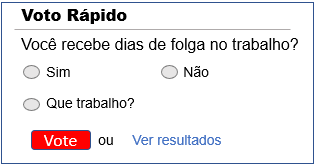
\includegraphics[width=0.5\textwidth]{1-3_data_collection_principles/vol_resp_bias_q.png}\pause
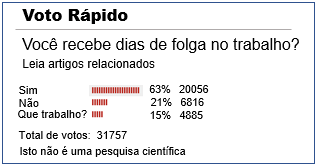
\includegraphics[width=0.5\textwidth]{1-3_data_collection_principles/vol_resp_bias_res.png} \\
{\tiny cnn.com, Jan 14, 2012}
\end{center}
\begin{itemize}
\pause
\justifying
\item \hl{Amostra de conveniência:} Indivíduos que são facilmente acessíveis têm maior probabilidade de serem incluídos na amostra.

\end{itemize}

\end{frame}

%%%%%%%%%%%%%%%%%%%%%%%%%%%%%%%%%%%%

\begin{frame}
\frametitle{Exemplo de viés de amostragem: Landon vs. FDR}
\justifying
Um exemplo histórico de uma amostra parcial que gera resultados enganosos: \\

$\:$ \\

\begin{columns}[c]

\column{0.35\textwidth}

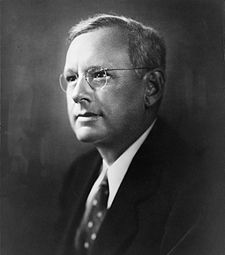
\includegraphics[width= \textwidth]{1-3_data_collection_principles/figures/landon_fdr/landon.png}

\column{0.3\textwidth}
\justifying
Em 1936, Landon buscou a indicação presidencial republicana contra a reeleição de FDR.

\column{0.35\textwidth}

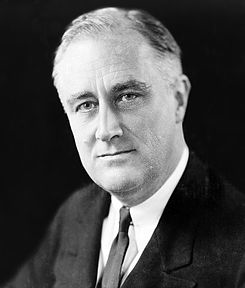
\includegraphics[width= \textwidth]{1-3_data_collection_principles/figures/landon_fdr/fdr.png}

\end{columns}

\end{frame}

%%%%%%%%%%%%%%%%%%%%%%%%%%%%%%%%%%%%%

\begin{frame}
\frametitle{A pesquisa de resumo literário}

\begin{columns}

\column{0.7\textwidth}

\begin{itemize}
\justifying
\item A revista Literary Digest entrevistou cerca de 10 milhões de americanos e obteve respostas de cerca de 2,4 milhões.
\justifying
\item A pesquisa mostrou que Landon provavelmente seria o grande vencedor da eleição e FDR receberia apenas 43 \% dos votos.

\item Resultado das eleições: FDR venceu com 62 \% dos votos.

\end{itemize}

\column{0.3\textwidth}

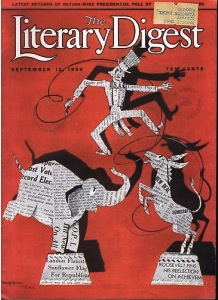
\includegraphics[width= \textwidth]{1-3_data_collection_principles/figures/literaryDigest.png}

\end{columns}

\begin{itemize}
\justifying
\item A revista ficou completamente desacreditada por causa da pesquisa e logo foi descontinuada.

\end{itemize}

\end{frame}

%%%%%%%%%%%%%%%%%%%%%%%%%%%%%%%%%%%%%

\begin{frame}
\frametitle{Sobre a pesquisa da revista Literary Digest - o que deu errado?}

\begin{itemize}

\item A revista havia pesquisado

\begin{itemize}

\item seus próprios leitores,

\item proprietários de automóveis registrados, e

\item usuários de telefone registrados.

\end{itemize}
\justifying
\item Esses grupos tinham rendimentos bem acima da média nacional da época (lembre-se, essa é a era da Grande Depressão) o que resultou em uma amostra de eleitores muito mais propensos a apoiar Landon, o que não representava o perfil eleitoral, ou seja, a amostra não era representativa da população americana na época.

\end{itemize}

\end{frame}

%%%%%%%%%%%%%%%%%%%%%%%%%%%%%%%%%%%%%

\begin{frame}
\frametitle{Amostras grandes são preferíveis, mas...}

\begin{itemize}
\justifying
\item A pesquisa eleitoral da Literary Digest  baseou-se em um tamanho de amostra de 2,4 milhões, o que é enorme, mas como a amostra era \bl {tendenciosa}, a amostra não produziu uma boa previsão.
\justifying
\item De volta à analogia da sopa: Se a sopa não estiver bem misturada, não importa quão grande seja a colher, ela ainda não terá o sabor certo. Se a sopa estiver bem misturada, uma colher pequena será suficiente para testar a sopa.

\end{itemize}

\end{frame}

%%%%%%%%%%%%%%%%%%%%%%%%%%%%%%%%%%%%%

\begin{frame}
\frametitle{Prática}
\justifying

\pq{Uma escola está considerando se permitirá que pais de alunos estacionem seus veículos na escola, depois de dois acidentes recentes. Como primeiro passo, eles enviam um e-mail aos pais e mães dos alunos, questionando se eles apoiariam essa mudança de política. De 6.000 e-mails, 1.200 são respondidos. Desses 1.200, 960 concordaram com a mudança de política e 240 discordaram. Qual das seguintes afirmações são verdadeiras?}
\end{frame}
%%%%%%%%%%%%%%%%%%%%%%%%%%%%%%%%%%%%%

\begin{frame}[shrink]
\frametitle{Prática}
\begin{enumerate}[I.]
\justifying
\item Alguns dos e-mails nunca foram recebidos pelos pais e pelas mães.
\justifying
\item Há forte concordância entre as famílias dos alunos, não deve-se permitir que estacionem o veículo  na escola.
\justifying
\item É possível que a maioria dos pais de alunos não esteja de acordo com essa mudança.
\justifying
\item É improvável que os resultados da pesquisa sejam parciais porque todos os pais receberam um e-mail.
\end{enumerate}


\justifying
\begin{multicols}{2}
\begin{enumerate}[(a)]
\item Somente I
\item I e II
\solnMult{I e III}
\item III e IV
\item Somente IV
\end{enumerate}
\end{multicols}


\end{frame}

%%%%%%%%%%%%%%%%%%%%%%%%%%%%%%%%%%%%%

\subsection{Variáveis explicativas e resposta}

%%%%%%%%%%%%%%%%%%%%%%%%%%%%%%%%%%%%%

\begin{frame}
\frametitle{Variáveis explicativas e de resposta}

\begin{itemize}
\justifying

\begin{center}
Variável explicativa $\xrightarrow{pode~afetar}$ variável resposta
\end{center}
\justifying
\item Rotular as variáveis como explicativas e respostas não garante que a relação entre as duas seja realmente causal, mesmo se houver uma associação identificada entre as duas variáveis. 

\end{itemize}

\end{frame}

%%%%%%%%%%%%%%%%%%%%%%%%%%%%%%%%%%%%%

\subsection{Estudos observacionais e experimentos aleatorizados}

%%%%%%%%%%%%%%%%%%%%%%%%%%%%%%%%%%%%%

\begin{frame}
\frametitle{Estudos observacionais e experimentos}

\begin{itemize}
\justifying
\item \hl{Estudos observacionais:} Os pesquisadores coletam dados de uma forma que não interfere diretamente na forma como os dados surgem, ou seja, eles apenas "observam", a interpretação dos resultados indicam associação entre as variáveis explicativas e respostas. Para avaliar a relação de causa e efeito é necessário estudos mais complexos, por meio de inferência causal. Essas técnicas não serão abordadas nesse curso.

\pause
\justifying
\item \hl{Experimentos:} Pesquisadores atribuem aleatoriamente sujeitos a vários tratamentos, a fim de estabelecer conexões causais entre as variáveis explicativas e de resposta.

\pause
\justifying
\item Lembre-se "correlação não implica causalidade".
\end{itemize}
\end{frame}
%%%%%%%%%%%%%%%%%%%%%%%%%%%%%%%%%%%%%

\begin{frame}
\frametitle{Estudos observacionais e experimentos}

\begin{center}
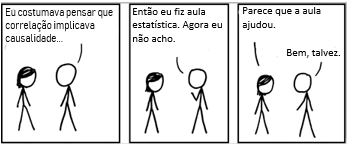
\includegraphics[width=0.7\textwidth]{1-3_data_collection_principles/xkcd_correlation.png} \\
{\tiny \webURL{http://xkcd.com/552/}}
\end{center}

\end{frame}

%%%%%%%%%%%%%%%%%%%%%%%%%%%%%%%%%%%%%

